
\section{Analysis of Moving Object Processing System Performance \label{sec:mops}}


The linking of individual detections from difference images into plausible orbital tracks will be performed using
a special-purpose code referred to as the Moving Object Processing System (MOPS). There are several slightly modified
versions of MOPS in use by various projects; the original version was developed collaboratively by Pan-STARRS
and LSST, and is described in \cite{denneau13}. MOPS employs a two-step processing: first pairs of detections
from a given night are connected into {\it tracklets}, and then at least three tracklets are associated into a
candidate {\it track}. Realistic MOPS simulations show high linking efficiency ($>$99\%; \citealt{denneau13})
across all classes of Solar System objects. The core algorithmic components of MOPS are {\it findTracklets} and
{\it linkTracklets} kd-tree algorithms by \citet{kubica07}. {\it findTracklets} links \DIASources from a single
night to produce {\it tracklets}, and {\it linkTracklets} links tracklets from at least three nights to produce candidate
{\it tracks} (assuming quadratic motion in each coordinate; the LSST version also accounts for topocentric
corrections). Candidate tracks produced by MOPS are then filtered using initial orbital determination (IOD) step,
which is executed using a stand-alone code (e.g. OrbFit, \citealt{milani08}; OpenOrb, \citealt{OpenOrb2009}).

Given empirically estimated false positive rates expected for LSST, discussed in the preceeding section,
in this section we show that MOPS performance is already adequate - MOPS requires significantly less
computing capacity than planned for other LSST data processing needs. In addition to reporting the results of
numerical experiments with MOPS, we also analyze them using analytic and semi-analytic results for the
rates of false tracklets and false tracks.




\subsection{A Summary of LSST tests of MOPS}

As a part of the Final Design Review preparations, the LSST team has developed an enhanced prototype
implementation of MOPS and analyzed its behavior. Here we summarize the main results of that work;
a detailed report is publicly available \citep{LDM-156}.

Simulated \DIASources were based on a Solar System model by \citet{Grav2011}.
The model includes about 11 million objects; about 9 million are main-belt asteroids. Observations span
30 days and were selected from a simulated baseline cadence (at that time, the baseline simulation was
OpSim3.61, which in this context is statistically the same as the current baseline cadence, {\it minion\_1016}).
The number of tracklets and tracks, the runtime, and the memory usage were studied as functions of
the false positive detection rate. The rate was varied from none to four times the asteroid detection rate
(100 deg$^{-2}$).  The highest rate corresponds to the expected false positive detection rate for LSST
($\rho_{FP} =  400$ deg$^{-2}$).

Tests were run with 16 threads on single 16 CPU node on Gordon cluster at San Diego Supercomputing
Center (in 2011). Due to computational constraints, a $v < 0.5$ deg/day velocity limit for pairing detections
into tracklets was imposed. For similar reasons, the filters that were imposed on track fitting were not
optimized, artificially reducing the yield. As we now understand the algorithmic scalings much better
(see Appendix~\ref{sec:appMOPS}), it is clear that these unoptimized filters have no major impact on the
simulation results and derived conclusions.

As expected, the addition of false positive detections increases the number of tracklets and tracks,
the runtime, and the memory usage. For the 4:1 false:true detection rate ratio, compared to case with
no false positive detections, the number of tracklets increases by about
a factor of 10, the number of tracks by about 50\%, and runtime increases by about a factor of 3.
For the 4:1 false:true detection rate ratio, the runtime with 16 CPUs is 33 hours, with maximum memory
usage of about 80 GB.




\begin{figure}[t!]
\centering
\vskip -0.3in
%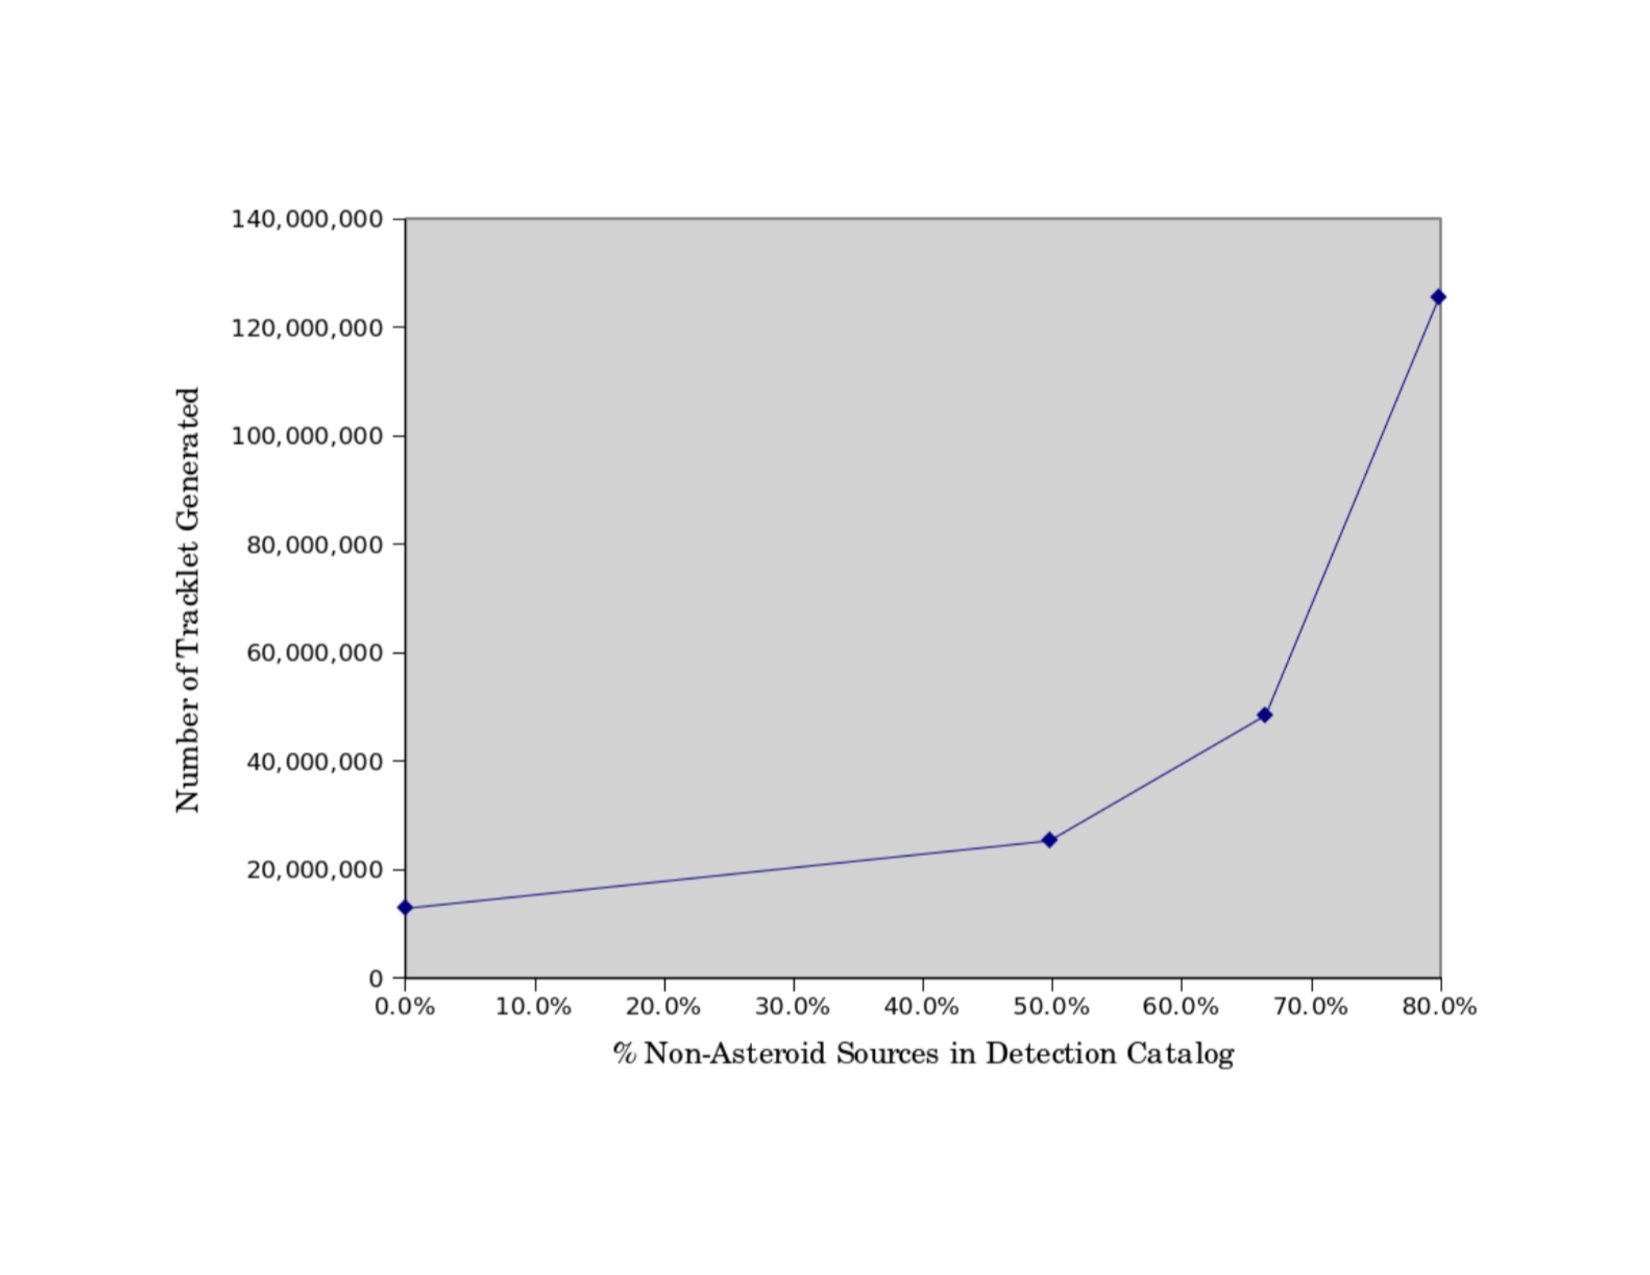
\includegraphics[width=0.49\textwidth]{figures/tracklet}
%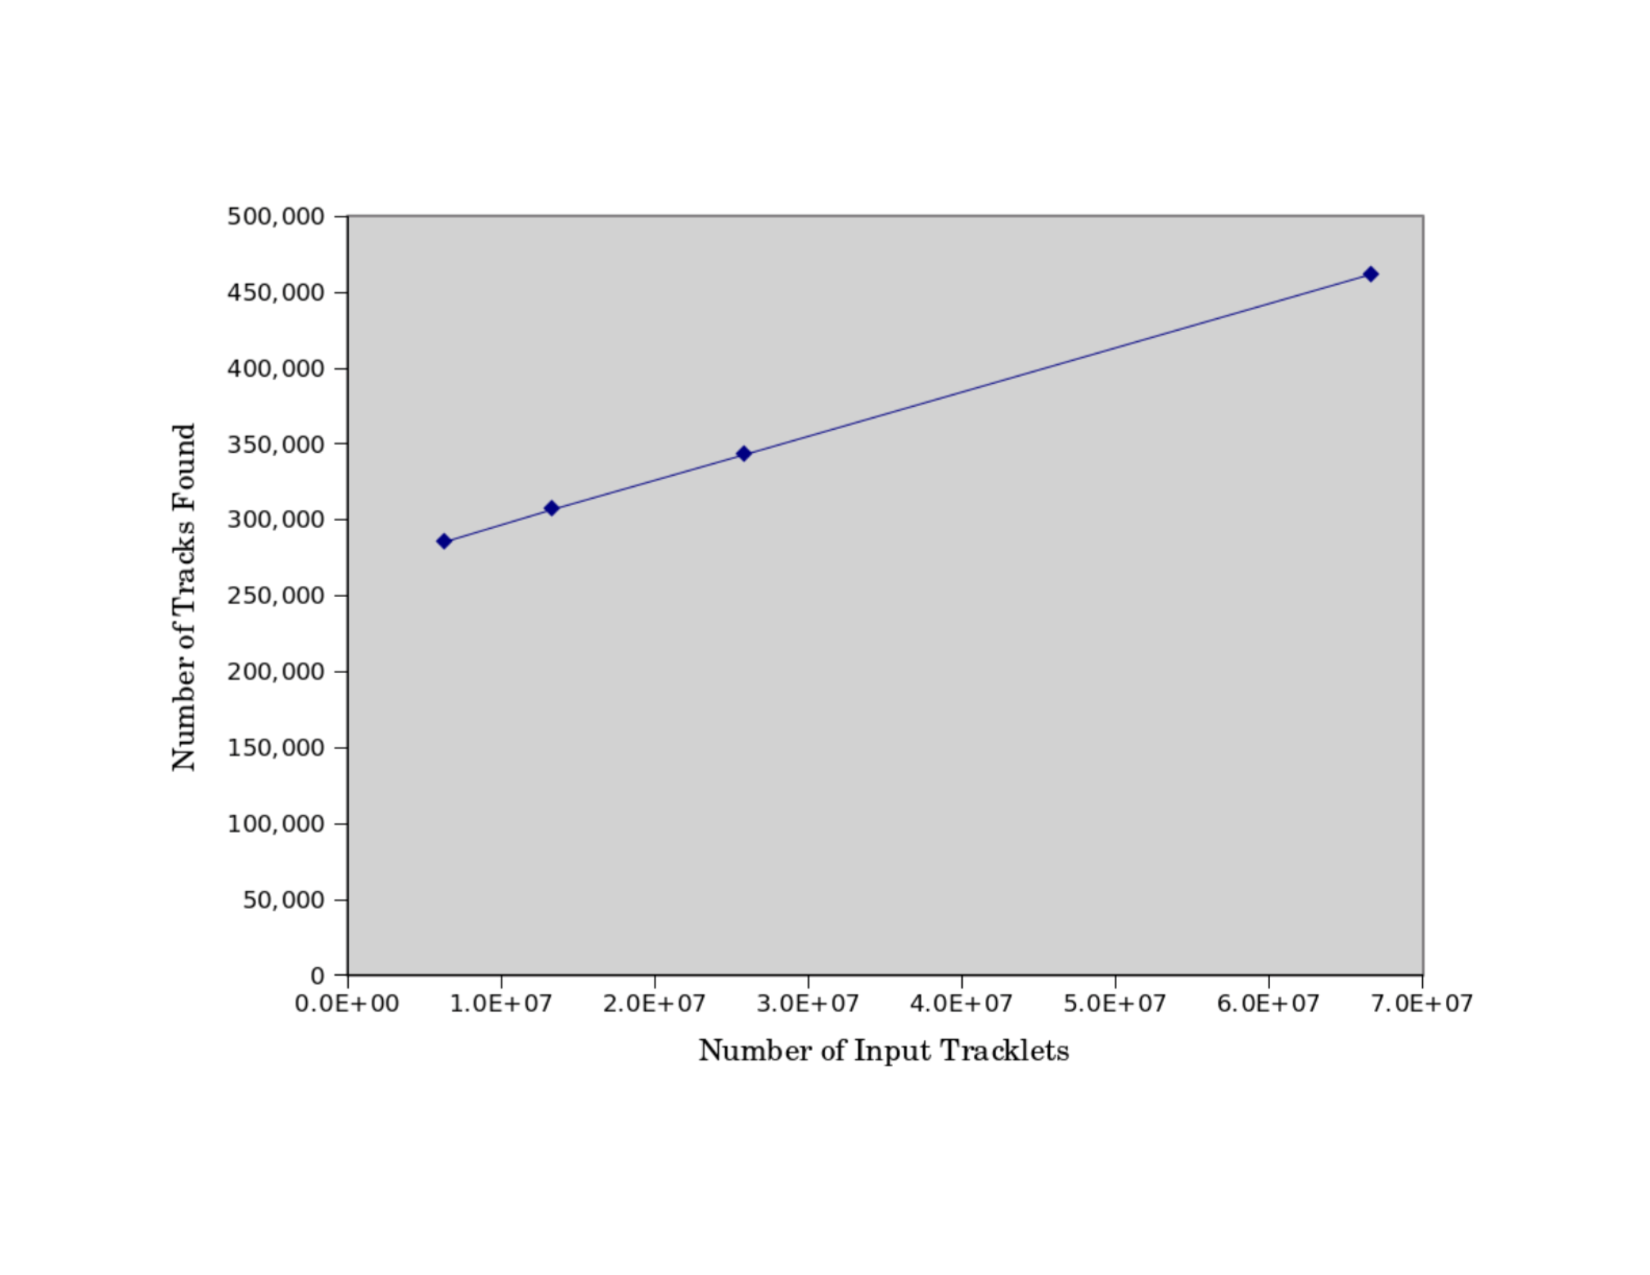
\includegraphics[width=0.49\textwidth]{figures/tracks}
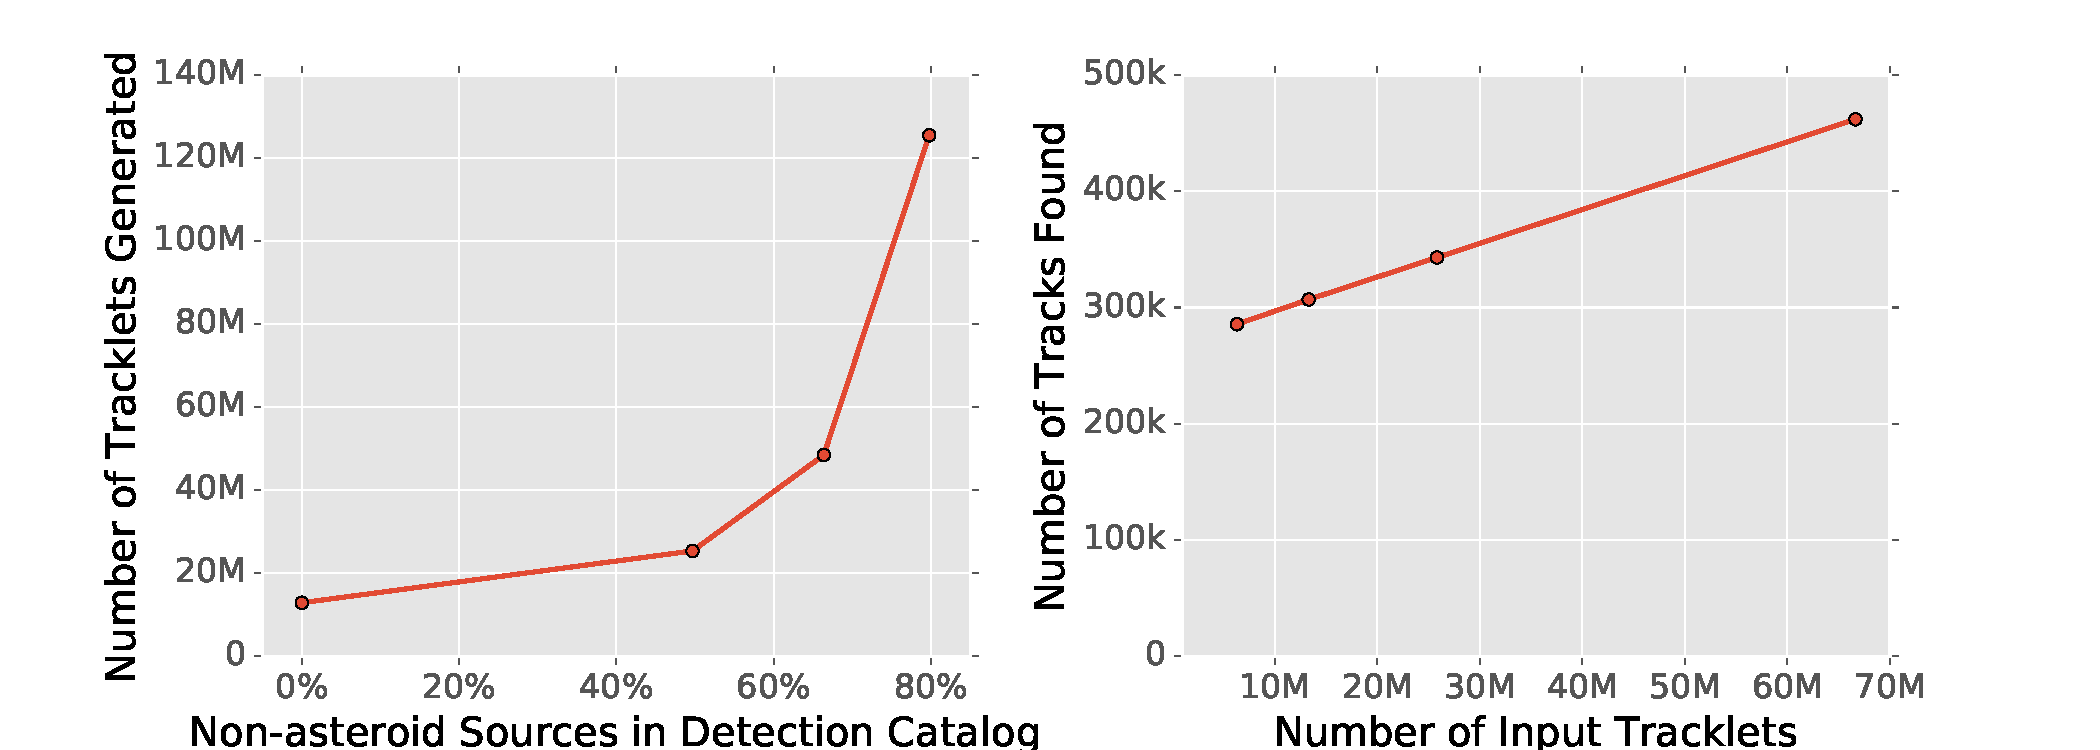
\includegraphics[width=0.95\textwidth]{figures/track_stats}
\caption{A summary of MOPS tests for the dependence of the number of tracklets (left)
and tracks (right) on the false positive detection rate. As the rate of false positive detections
increases from none to four times the asteroid detection rate, the number of tracklets
increases by about an order of magnitude. At the same time, the number of candidate
tracks increases by only about 50\%.
\label{fig:MOPStests}}
\end{figure}




\subsection{Understanding MOPS Performance}

The rather slow increase of the number of tracks with false positive detection rate (only 50\% increase
although the number of tracklets increased by a factor of 10) is somewhat unexpected. We have
developed analytic and semi-analytic analysis to better understand the scaling of the number of
tracklets and tracks with false positive detection rate and other relevant parameters. Details of this
analysis are provided in Appendix~\ref{sec:appMOPS}. Here we briefly discuss the main results.

The increase of the number of tracklets with false positive detection rate,
$\rho_{FP}$, shown in left panel in Figure~\ref{fig:MOPStests}, is well
described by eq.~\ref{eq:NttFalse}. In particular, the number of tracklets
approximately increases proportionally to $(C_1 + C_2\rho_{FP}^2)$, where $C_1$
and $C_2$ do not depend on $\rho_{FP}$. As both the full analytic result and the
simulations show, false tracklets quickly outnumber true tracklets even at low
false detection rates, resulting in the observed $\rho_{FP}^2$ behavior.

While the number of tracklets is dominated by the false positive detections, in
baseline LSST cadence and nominal noise assumptions under which the MOPS
simulations were run ($\rho_{FP} \leq 500\,\rm{deg}^{-2}$), the number of
tracks is not dominated by spurious detections---instead it is dominated by true
tracks and mislinkages between true objects. This is due to the fundamental
feature of MOPS: the 4-dimensional space of tracks (two coordinates and two
velocity vector components) is sparse at up to moderate levels of contamination,
and at the tested noise levels false tracklets are effectively filtered. This
behavior accounts for the slow growth in tracks in the right panel of
Figure~\ref{fig:MOPStests}.

As we evaluate the impact of different survey parameters, we can assess the
number of tracks that would be generated (and thus require IOD processing) using
the analytic results developed in Appendix~\ref{sec:appMOPS}. For a given window
width and false detection density, the number of false tracks per search window
that would arise from false detections is given by
\begin{equation}
\label{eq:falsetracks2}
   N^{falsetracks} = 4.5 \times 10^6 \, \left( {N_w \over 30 \, {\rm day} } \right)^{8} \left( {\rho_{FP} \over 400 \, {\rm deg}^{-2} }\right)^{3.7}.
\end{equation}
This expression is valid around fiducial values and assumes $\rho_{ast}=100$ deg$^{-2}$.
The number of true tracks is of the order 10$^6$; therefore, with the baseline
window $N_W=15$ the contribution of false detections is small, while in the
enhanced NEO cadences with $N_W=30$ the contribution is only a factor of a few
times the number of true tracks.

\subsection{Required Computing Resources for MOPS and IOD Processing}

Given the modest computing resources used in MOPS tests described above, the runtime and memory
usage results bode well for LSST processing. Assuming a 1000-core machine dedicated to LSST moving
object processing (corresponding to about 1\% of the anticipated total LSST compute power at the
National Center for Supercomputing Applications), MOPS runtime for producing
candidate tracks should not exceed an hour, assuming sufficient parallelization can be achieved.

The IOD step can also be handled with anticipated resources and is trivially parallelizable. The number 
of available IOD computations for a system a compute system with $N_{core}$ cores and allocated runtime $T_{runtime}$ can be estimated
as
\begin{equation}
  N_{IOD} = 3.6\times10^8 \left({ 0.1\,{\rm sec} \over T_{IOD}}\right) \,
                                         \left({ T_{runtime}  \over 10\,{\rm hr} }\right) \,
                                         \left({ N_{core}  \over 1000}\right).
\end{equation}
where $T_{IOD}$ is the time it takes to perform one IOD computation on a single core. Estimates
of $T_{IOD}$ are in the range of 50 mas (S. Chesley, priv. comm.), considerably below the fiducial
value of 100 mas adopted here. Given that the expected number of candidate tracks to filter using
IOD is well below $10^7$, it should be possible to accomplish the IOD step in well under an hour.
Alternatively, it is plausible that a 100-core machine might be sufficient for LSST moving object
processing (assuming no engineering safety margin).
